% TEMPLATE.TEX
%
% Time-stamp: <2013-03-26 11:09 olenz>
%
% This is an extensively documented LaTeX file that shows how to
% produce a good-looking document with current LaTeX (11/2012).
%
% IMPORTANT!
%
%   Some obsolete commands and packages
% ----------|-------------------------------
% obsolete  |     Replacement in LATEX 2ε
% ----------|-------------------------------
%           | local            global/switch
% ----------|-------------------------------
% {\bf ...} | \textbf{...}     \bfseries
%     -     | \emph{...}       \em
% {\it ...} | \textit{...}     \itshape
%     -     | \textmd{...}     \mdseries
% {\rm ...} | \textrm{...}     \rmfamily
% {\sc ...} | \textsc{...}     \scshape
% {\sf ...} | \textsf{...}     \sffamily
% {\sl ...} | \textsl{...}     \slshape
% {\tt ...} | \texttt{...}     \ttfamily
%     -     | \textup{...}     \upshape
%
% DON'T USE \\ TO MAKE LINEBREAKS, INSTEAD JUST LEAVE A BLANK LINE!
%
\RequirePackage[l2tabu,orthodox]{nag} % turn on warnings because of bad style
\documentclass[a4paper,10pt,bibtotoc]{scrartcl}
%
\usepackage[bottom=3.5cm, top=3cm]{geometry}
\usepackage{subcaption}
\captionsetup[subfigure]{list=true, position=top}
\usepackage{float}
%%%%%%%%%%%%%%%%%%%%%%%%%%%%%%%%%%%%
% KOMA CLASSES
%%%%%%%%%%%%%%%%%%%%%%%%%%%%%%%%%%%%
%
% The class "scrartcl" is one of the so-called KOMA-classes, a set of
% very well done LaTeX-classes that produce a very European layout
% (e.g. titles with a sans-serif font).
%
% The KOMA classes have extensive documentation that you can access
% via the commands:
%   texdoc scrguide # in German
%   texdoc scrguien # in English
%
%
% The available classes are:
%
% scrartcl - for "articles", typically for up to ~20 pages, the
%            highest level sectioning command is \section
%
% scrreprt - for "reports", typically for up to ~200 pages, the
%            highest level sectioning command is \chapter
%
% scrbook  - for "books", for more than 200 pages, the highest level
%            sectioning command is \part.
%
% USEFUL OPTIONS
%
% a4paper  - Use a4 paper instead of the default american letter
%            format.
%
% 11pt, 12pt, 10pt
%          - Use a font with the given size.
%
% bibtotoc - Add the bibliography to the table of contents
%
% The KOMA-script classes have plenty of options to modify

% This allows to type UTF-8 characters like ä,ö,ü,ß
\usepackage[utf8]{inputenc}

\usepackage[T1]{fontenc}        % Tries to use Postscript Type 1 Fonts for better rendering
\usepackage{lmodern}            % Provides the Latin Modern Font which offers more glyphs than the default Computer Modern
\usepackage[intlimits]{amsmath} % Provides all mathematical commands
\usepackage{amssymb}
\usepackage{hyperref}           % Provides clickable links in the PDF-document for \ref
\usepackage{graphicx}            % Allow you to include images (like graphicx). Usage: \includegraphics{path/to/file}

% Allows to set units
\usepackage[ugly]{units}        % Allows you to type units with correct spacing and font style. Usage: $\unit[100]{m}$ or $\unitfrac[100]{m}{s}$

% Additional packages
\usepackage{url}                % Lets you typeset urls. Usage: \url{http://...}
\usepackage{breakurl}           % Enables linebreaks for urls
\usepackage{xspace}             % Use \xpsace in macros to automatically insert space based on context. Usage: \newcommand{\es}{ESPResSo\xspace}
\usepackage{xcolor}             % Obviously colors. Usage: \color{red} Red text
\usepackage{booktabs}           % Nice rules for tables. Usage \begin{tabular}\toprule ... \midrule ... \bottomrule
\usepackage{siunitx}


% Source code listings
\usepackage{listings}           % Source Code Listings. Usage: \begin{lstlisting}...\end{lstlisting}
\lstloadlanguages{python}
\definecolor{lightpurple}{rgb}{0.8,0.8,1}

\lstset{
stepnumber=1,
numbersep=5pt,
numberstyle=\small\color{black},
basicstyle=\ttfamily,
%keywordstyle=\color{black},
%commentstyle=\color{black},
%stringstyle=\color{black},
frame=single,
tabsize=4,
language = python,
backgroundcolor=\color{black!5}}

\usepackage{float}

\begin{document}

\titlehead{Simulation Methods in Physics I \hfill WS 2019/2010}
\title{Report for Worksheet 3: Molecular Dynamics 2 and Observables}
\author{Markus Baur and David Beyer}
\date{\today}
%\publishers{Institute for Computational Physics, University of Stuttgart}
\maketitle

\tableofcontents
\newpage

\section{Saving and Restarting the Simulation}
The state of a previous simulation is loaded in this fashion from the checkpoint file:
\begin{lstlisting}
else:
    logging.info("Reading state from checkpoint.")
    with open(args.cpt, 'rb') as fp:
    state = pickle.load(fp)
    positions = state['positions']
    energies = state['energies']
    pressures = state['pressures']
    temperatures = state['temperatures']
    rdfs = state['rdfs']
    potential_energies = state['potential_energies']
    kinetic_energies = state['kinetic_energies']

    x = state['x']
    v = state['v']
    f = state['f']
    f_max = state['f_max']
\end{lstlisting}
During the simulation, these observables are measured:
\begin{lstlisting}
for i in tqdm.tqdm(range(N_TIME_STEPS)):
    sim.propagate()

    if i % SAMPLING_STRIDE == 0:
        positions.append(sim.x.copy())
        pressures.append(sim.pressure())
        energies.append(np.sum(sim.energy()))
        temperatures.append(sim.temperature())
        rdfs.append(sim.rdf())
        potential_energies.append(sim.e_pot())
        kinetic_energies.append(sim.e_kin())
\end{lstlisting}
These observables are written to the checkpoint file in the end:
\begin{lstlisting}
if args.cpt:
    state = {'positions': positions,
             'energies': energies,
             'pressures': pressures,
             'temperatures': temperatures,
             'rdfs': rdfs,
             'potential_energies': potential_energies,
             'kinetic_energies': kinetic_energies,
             'x':sim.x,
             'v': sim.v,
             'f': sim.f,
             'f_max': sim.f_max}
    write_checkpoint(state, args.cpt, overwrite=True)
\end{lstlisting}

\newpage
\section{Simple Observables}
The kinetic energy is calculated from the velocities:
\begin{lstlisting}
def e_kin(self):
    return np.sum(0.5 * np.power(self.v, 2))  # mass = 1
\end{lstlisting}
The potential energy can be calculated as the sum of the entries of the array e\_pot\_ij\_matrix.
Because every pair is summed over twice, a factor of 0.5 is needed:
\begin{lstlisting}
def e_pot(self):
    return np.sum(self.e_pot_ij_matrix) / 2
\end{lstlisting}
The function energy returns a NumPy array which contains the potential and kinetic energy:
\begin{lstlisting}
def energy(self):
    self.energies()

    return np.array((self.e_pot(), self.e_kin()))
\end{lstlisting}
The temperature of the system is calculated using the equipartition theorem, it is implemented in this way:
\begin{lstlisting}
def temperature(self):
    return 2 * self.e_kin() / (self.n_dims * self.n)
\end{lstlisting}
The pressure is calculated using the formula given in the lecture/on the worksheet:
\begin{lstlisting}
def pressure(self):
    f = np.multiply(self.f_ij_matrix, self.r_ij_matrix)
    f = np.sum(f)

    area = np.product(self.box)
    ret = 1 / area * (self.e_kin() + f * 0.25)
    return ret
\end{lstlisting}
The sum $\sum_{i<j}\langle\mathbf{r}_{ij}\cdot\mathbf{F}_{ij}\rangle$ is calculated as a pointwise multiplication and subsequent summation of the arrays f\_ij\_matrix and r\_ij\_matrix. 
Because the sum only runs over $i<j$, an additional factor of 0.5 is needed.

\newpage
\section{Equilibration}
\autoref{fig:fig1} shows the time evolution the potential energy $E_\mathrm{pot}$, kinetic energy $E_\mathrm{kin}$, pressure $P$ and temperature $T$ for a total time of 1000 time steps.
We can see that all of them exhibit a time drift. 
\autoref{fig:fig2} shows the time evolution of the same observables for a total time of 100000 time steps.
We can see that after an initial time-drift they seem to fluctuate around constant values.
\begin{figure}[H]
        \centering
        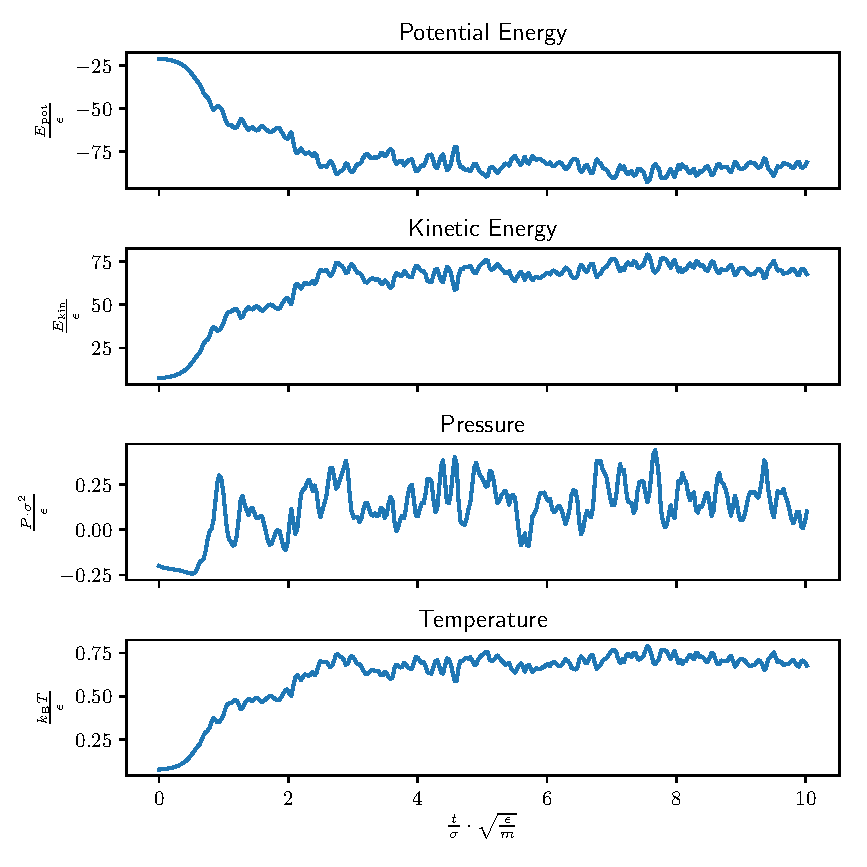
\includegraphics[width=\linewidth]{Figure_1.pdf}
    \caption{Time evolution of the potential energy $E_\mathrm{pot}$, kinetic energy $E_\mathrm{kin}$, pressure $P$ and temperature $T$ for a total time of 1000 time steps.}
    \label{fig:fig1}
\end{figure}
\begin{figure}[H]
        \centering
        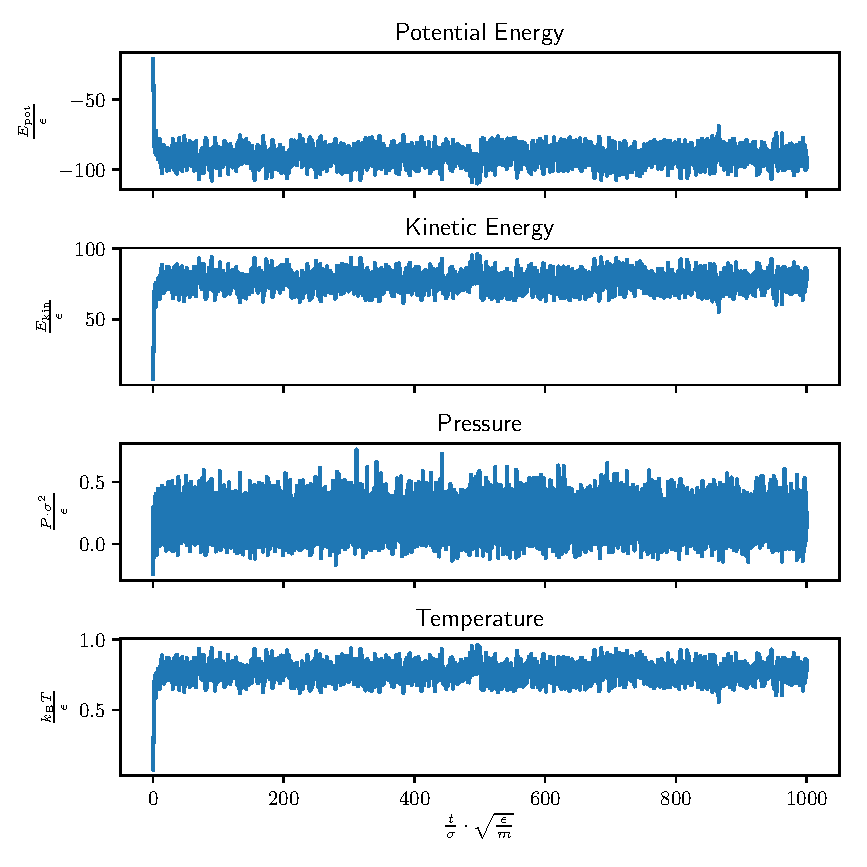
\includegraphics[width=\linewidth]{Figure_2.pdf}
    \caption{Time evolution of the potential energy $E_\mathrm{pot}$, kinetic energy $E_\mathrm{kin}$, pressure $P$ and temperature $T$ for a total time of 100000 time steps.}
    \label{fig:fig2}
\end{figure}
The function to calculate the running average of an observable is implemented in this fashion:
\begin{lstlisting}
def running_average(O, M):
    ret = np.empty_like(O)
    N = len(O)
    for i in range(0, N):
        if (i < M) or (i >= N - M):
            ret[i] = np.nan
        else:
            ret[i] = np.sum(O[i-M:i+M+1]) / (2*M + 1)
    return ret
\end{lstlisting}
The function has as its arguments the time series of the observable O in the form of a NumPy array as well as the window size. 
It returns a NumPy array of the same size as the original time series, for all times for which the running average cannot be calculated, the value is set to np.nan. 
To sum all values in the window, the NumPy function np.sum is used.

\autoref{fig:fig3} shows the time evolution of the observables for a total time of 100000 time steps.
Furthermore, the running averages are shown for window sizes of $M=10$ and $M=100$.
We can see that the running averages fluctuate less than the raw data and that the running average for $M=100$ fluctuates less than the one for $M=10$.
The initial time drift of the observables corresponds to the equilibration of the system, it takes place on a time scale of about
\begin{align*}
t_\mathrm{eq}\approx 10\cdot\sigma\cdot\sqrt{\frac{m}{\epsilon}}.
\end{align*}
After this equilibration time, the observables fluctuate around approximately constant values.
\begin{figure}[H]
        \centering
        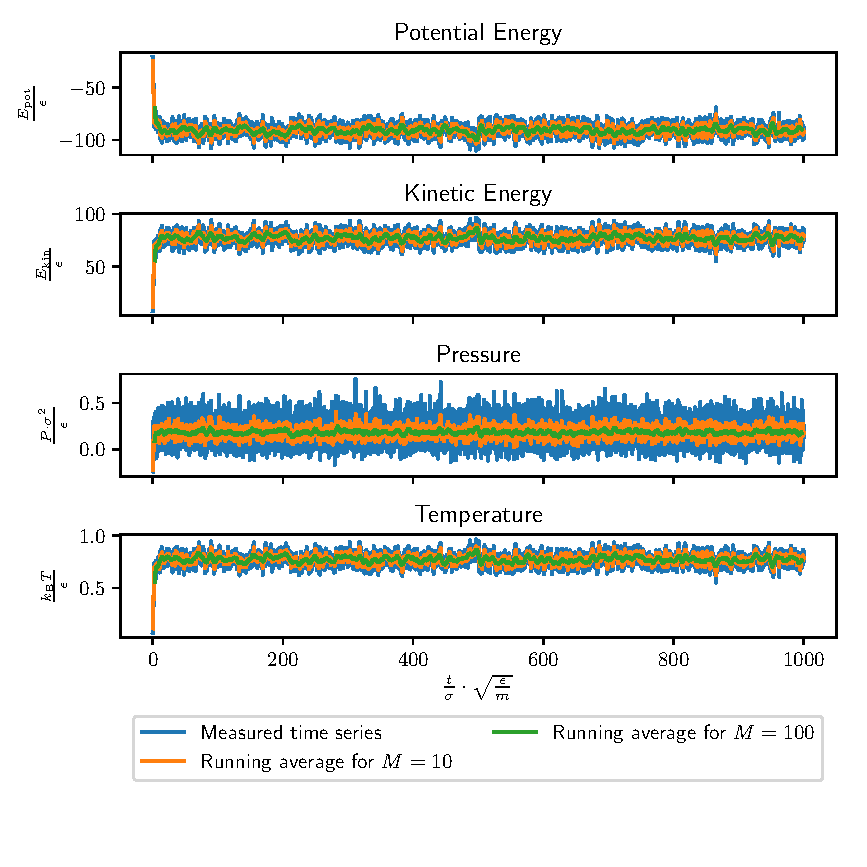
\includegraphics[width=\linewidth]{Figure_3.pdf}
    \caption{Time evolution of the potential energy $E_\mathrm{pot}$, kinetic energy $E_\mathrm{kin}$, pressure $P$ and temperature $T$ for a total time of 1000 time steps as well as the running averages for window sizes of $M=10$ and $M=100$.}
    \label{fig:fig3}
\end{figure}
To compute the mean values of the observables after an equilibration time $t_\mathrm{eq}$, the function print\_teq() was added:
\begin{lstlisting}
def print_teq():
    if not hasattr(args, "t_eq"):
        return
    for o in observables:
        d = data[o]
        d = d[args.t_eq:]
        print("Average equilibrium %s: %s" % (o, sum(d) / len(d)))
\end{lstlisting}
The function contains a for-loop which runs over all observables and computes their equilibrium mean value (mean value from $t_{eq}$ to the end of measurement) and outputs it.
The measured equilibrium mean values are:
\begin{align*}
\left\langle E_\mathrm{pot}/\epsilon \right\rangle &\approx  -90.63\\
\left\langle E_\mathrm{kin}/\epsilon\right\rangle &\approx 77.06\\
\left\langle \frac{P\sigma ^2}{\epsilon}\right\rangle &\approx 0.1831\\
\left\langle \frac{k_\mathrm{B}T}{\epsilon}\right\rangle &\approx 0.7706.
\end{align*}

\newpage
\section{Molecular Dynamics at a Desired Temperature}
The temperature $T(t)$ of the system at a given time $t$ is given by the equipartition theorem:
\begin{align}
T(t) = \frac{1}{k_\mathrm{B}DN}\sum_{i=1}^{N}\frac{m}{2}\mathbf{v}^2.
\end{align}
To reach the desired temperature $T_0$, we introduce rescaled velocities:
\begin{align}
\mathbf{v}\rightarrow a\cdot\mathbf{v}
\end{align}
with a scaling factor $a$. 
This results in
\begin{align}
T_0 = \frac{1}{k_\mathrm{B}DN}\sum_{i=1}^{N}\frac{m}{2}\left(a\cdot\mathbf{v}\right)^2 =a^2\cdot \frac{1}{k_\mathrm{B}DN}\sum_{i=1}^{N}\frac{m}{2}\mathbf{v}^2 = a^2\cdot T(t).
\end{align}
We can identify the scaling factor $a$ as
\begin{align}
a = \sqrt{\frac{T_0}{T(t)}}.
\end{align}
The rescaling function looks like this:
\begin{lstlisting}
def rescale(self, T0):
        temp = self.temperature()
        factor = np.sqrt(T0 / temp)
        self.v *= factor
\end{lstlisting}
This function is then called every time the observables are measured. The velocity rescaling can be enabled with the command line option -t [$T_0$].

The time evolution of the potential energy $E_\mathrm{pot}$, kinetic energy $E_\mathrm{kin}$, pressure $P$ and temperature $T$ for a total time of 210000 time steps as well as the running averages for window sizes of $M=10$ and $M=100$ are shown in \autoref{fig:fig4} -- \autoref{fig:fig6}. 
The simulations are first run for 10000 time steps with velocity rescaling and a target temperature of $T_0 = \{0.3, 1.0, 2.0\}\cdot \epsilon\cdot k_\mathrm{B}^{-1}$. 
Afterwards, the velocity rescaling is turned off and the time evolution is computed in the microcanonical ensemble for another 200000 time steps.
In the beginning of the simulation, we observe rapid changes in the energy components and the temperature, these are cause by the velocity rescaling.
We can see that the temperature and kinetic energy begin to fluctuate again when the velocity-rescaling-thermostat is turned off, this is expected since they are not rescaled every third step anymore.
Furthermore we observe that the potential energy decreases during the time when the velocity rescaling is used.
For a target temperature of $T_0 = 0.3\cdot \epsilon\cdot k_\mathrm{B}^{-1}$, the following equilibrium mean values were measured:
\begin{align*}
\left\langle E_\mathrm{pot}/\epsilon \right\rangle &\approx-221.4\\
\left\langle E_\mathrm{kin}/\epsilon\right\rangle &\approx 30.60\\
\left\langle \frac{P\sigma ^2}{\epsilon}\right\rangle &\approx -0.029\\
\left\langle \frac{k_\mathrm{B}T}{\epsilon}\right\rangle &\approx 0.306.
\end{align*}
For a target temperature of $T_0 = 1.0\cdot \epsilon\cdot k_\mathrm{B}^{-1}$, the following equilibrium mean values were measured:
\begin{align*}
\left\langle E_\mathrm{pot}/\epsilon \right\rangle &\approx-81.32\\
\left\langle E_\mathrm{kin}/\epsilon\right\rangle &\approx 102.0\\
\left\langle \frac{P\sigma ^2}{\epsilon}\right\rangle &\approx0.313\\
\left\langle \frac{k_\mathrm{B}T}{\epsilon}\right\rangle &\approx 1.020.
\end{align*}
For a target temperature of $T_0 = 2.0\cdot \epsilon\cdot k_\mathrm{B}^{-1}$, the following equilibrium mean values were measured:
\begin{align*}
\left\langle E_\mathrm{pot}/\epsilon \right\rangle &\approx-64.81\\
\left\langle E_\mathrm{kin}/\epsilon\right\rangle &\approx 203.6\\
\left\langle \frac{P\sigma ^2}{\epsilon}\right\rangle &\approx 0.839\\
\left\langle \frac{k_\mathrm{B}T}{\epsilon}\right\rangle &\approx 2.036.
\end{align*}
In all three cases the mean value of the measured temperature is close to the target temperature which was used for the velocity rescaling.
\begin{figure}
        \centering
        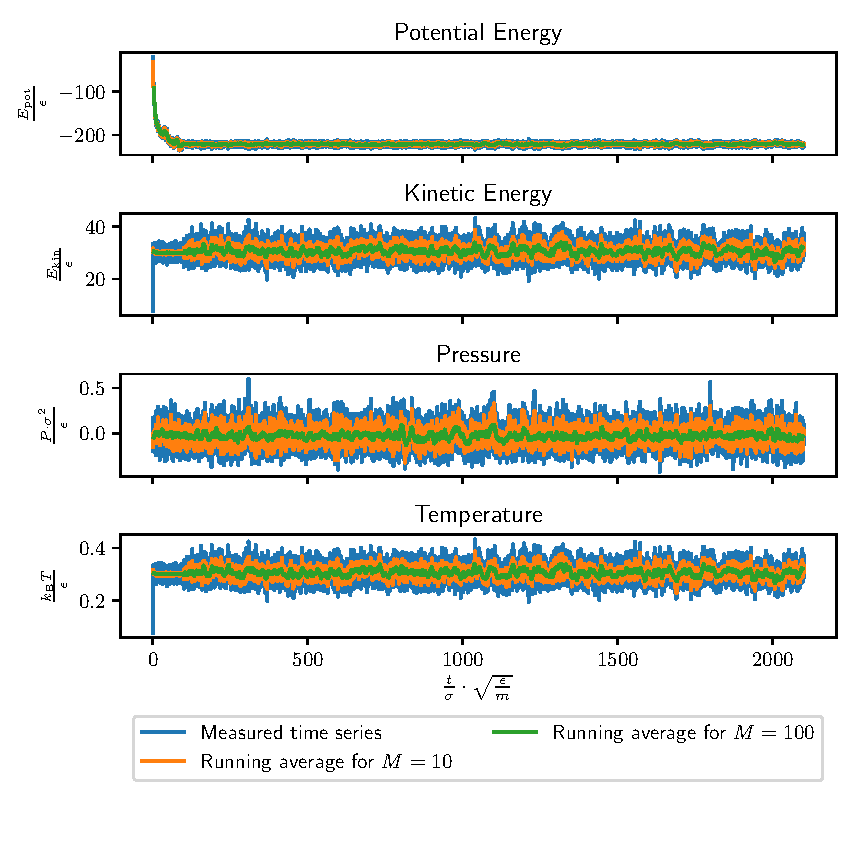
\includegraphics[width=\linewidth]{Figure_4.pdf}
    \caption{Time evolution of the potential energy $E_\mathrm{pot}$, kinetic energy $E_\mathrm{kin}$, pressure $P$ and temperature $T$ for a total time of 210000 time steps as well as the running averages for window sizes of $M=10$ and $M=100$. The simulation is first run for 10000 time steps with velocity rescaling and a target temperature of $T_0 = 0.3\cdot \epsilon\cdot k_\mathrm{B}^{-1}$. Afterwards, the velocity rescaling is turned off and the time evolution is computed in the microcanonical ensemble for another 200000 time steps.}
    \label{fig:fig4}
\end{figure}
\begin{figure}
        \centering
        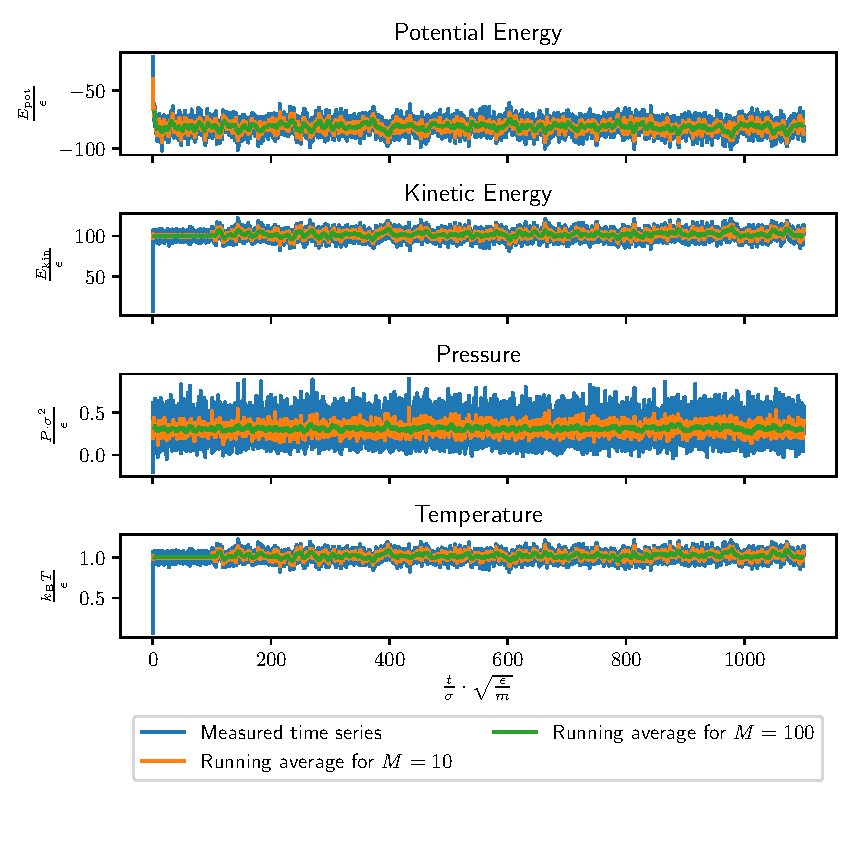
\includegraphics[width=\linewidth]{Figure_5.pdf}
    \caption{Time evolution of the potential energy $E_\mathrm{pot}$, kinetic energy $E_\mathrm{kin}$, pressure $P$ and temperature $T$ for a total time of 210000 time steps as well as the running averages for window sizes of $M=10$ and $M=100$. The simulation is first run for 10000 time steps with velocity rescaling and a target temperature of $T_0 = 1.0\cdot \epsilon\cdot k_\mathrm{B}^{-1}$. Afterwards, the velocity rescaling is turned off and the time evolution is computed in the microcanonical ensemble for another 200000 time steps.}
    \label{fig:fig5}
\end{figure}
\begin{figure}
        \centering
        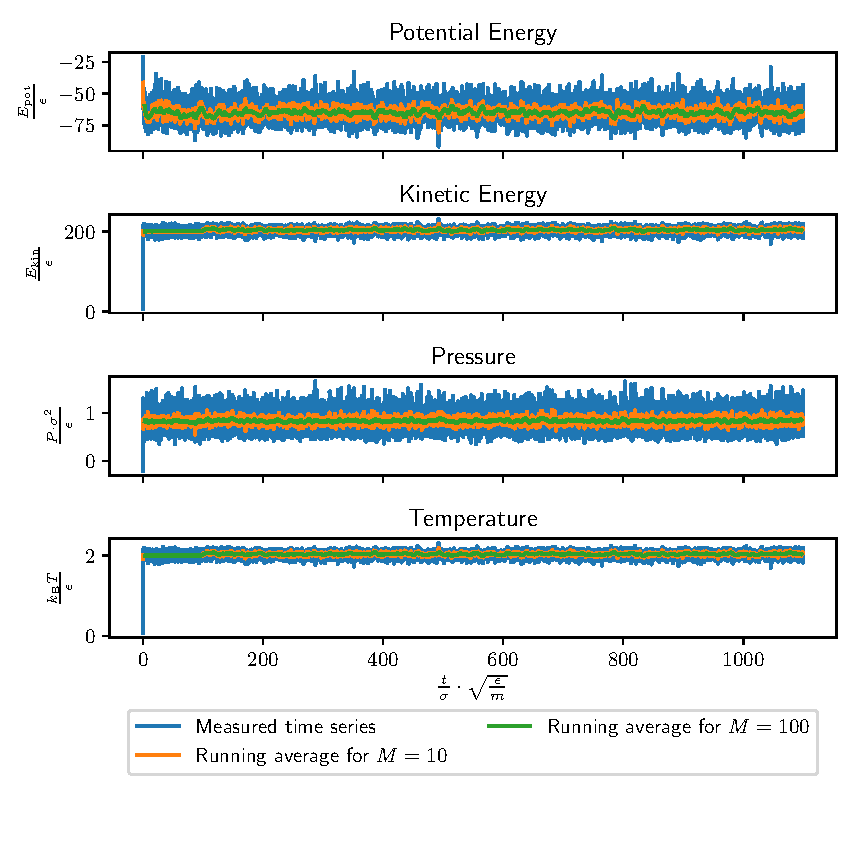
\includegraphics[width=\linewidth]{Figure_6.pdf}
    \caption{Time evolution of the potential energy $E_\mathrm{pot}$, kinetic energy $E_\mathrm{kin}$, pressure $P$ and temperature $T$ for a total time of 210000 time steps as well as the running averages for window sizes of $M=10$ and $M=100$. The simulation is first run for 10000 time steps with velocity rescaling and a target temperature of $T_0 = 2.0\cdot \epsilon\cdot k_\mathrm{B}^{-1}$. Afterwards, the velocity rescaling is turned off and the time evolution is computed in the microcanonical ensemble for another 200000 time steps.}
    \label{fig:fig6}
\end{figure}

\newpage
\section{Setting up and Warming up the System}
In order to enable force capping, the function which computes the forces is modified in the following way:
\begin{lstlisting}
def forces(self):
    # first update the distance vector matrix,
    # obeying minimum image convention
    self.distances()
    self.f_ij_matrix = self.r_ij_matrix.copy()
    r = np.linalg.norm(self.r_ij_matrix, axis=2)
    with np.errstate(all='ignore'):
        fac = np.where((r != 0.0) & (r < self.r_cut),\
        4.0 * (12.0 * np.power(r, -13.) - 6.0 * np.power(r, -7.)),\
        0.0)
    for dim in range(self.n_dims):
        with np.errstate(invalid='ignore'):
            self.f_ij_matrix[:, :, dim] *= np.where(r != 0.0,\
            fac / r,0.0)
    f = np.sum(self.f_ij_matrix, axis=0).transpose()
    self.f = np.clip(f, - self.f_max, self.f_max)
\end{lstlisting}
The NumPy function np.clip confines the force to the interval $[-f_\mathrm{max},f_\mathrm{max}]$.
When starting the simulation, an initial value for $f_\mathrm{max}$ can be set with the option $-f$. 
While the simulation is running, $f_\mathrm{max}$ is increase by 10\% every time the observables are measured:
\begin{lstlisting}
if args.fmax:
    sim.f_max *= 1.1
    if sim.f_max >= 1e9:
        sim.f_max = np.inf
\end{lstlisting}
Once a value of $f_\mathrm{max}=10^9$ is reached, the force capping is turned off.
To assign random initial particle positions, the following code is used.
\begin{lstlisting}
x = np.random.random((DIM, N_PART))
for i in range(DIM):
    x[i] *= BOX[i]
\end{lstlisting}
The warming up with force-capping and velocity rescaling works as intended, details are discussed in section 7.

\newpage
\section{Radial Distribution Function}
To calculate the radial distribution function at a given time, the following function was implemented:
\begin{lstlisting}
def rdf(self):
    self.distances()
    r = np.linalg.norm(self.r_ij_matrix, axis=2)
    hist, bins = np.histogram(r, bins=100, range=(0.8, 5))
    return hist
\end{lstlisting}
First, the distances are calculated from the matrix of distance vectors. 
Next, a histogram is produced using the NumPy function np.histogram. 
Note that this histogram is not properly normalized. 
Because we are only interested in the average RDF, the normalization is performed in the same step as the averaging.
The function to compute the average RDF beginning at a given time $t_\mathrm{eq}$ looks the following way:
\begin{lstlisting}
def average_rdf(rdfs, t_eq):
    rdfs = rdfs[t_eq:]
    ret = np.zeros_like(rdfs[0])
    for i in range(len(rdfs)):
        ret += rdfs[i]
    ret = ret/len(rdfs)
    for i in range(0, 100):
        ret[i] /= 100*np.pi*DENSITY*(2*dr*(0.8+i*dr) + dr*dr)
    return ret
\end{lstlisting}
First, all of the histograms beginning with $t_\mathrm{eq}$ are added. 
Then, the normalization is performed: first, the obtained histogram is divided by the total number of added histograms. 
Next, another normalization is performed in order to obtain an actual RDF.
The normalization can be derived the following way: The RDF measures, how many particles are in a radial bin $[r,r+\Delta r]$ compared to an ideal gas of the same average density.
The number of particles in the bin $[r,r+\Delta r]$ for an ideal gas of density $\rho$ is given by.
\begin{align}
N\left([r,r+\Delta r]\right) = \rho\cdot\int_{0}^{2\pi}\mathrm{d}\phi\int_{r}^{r+\Delta r}\mathrm{d}r'\, r' = \pi \rho\left(2r\Delta r + \Delta r^2\right).
\end{align}
In the function average\_rdf presented above there also appears an additional factor of $100$, this number corresponds to the total number of particles and accounts for the fact that the function rdf computes the histogram over all distances (average over all particles).

\newpage
\section{Measuring Equilibrium Mean Values of the Observables}
\subsection{$T = 0.3\cdot \epsilon\cdot k_\mathrm{B}^{-1}$}
To warm up the system with random initial positions, a simulation with an initial force capping of $f_\mathrm{max} = 20.0\cdot\epsilon\cdot \sigma^{-1}$ and velocity rescaling was run for 1000 time steps.
A plot of the observables during this warming up is shown in \autoref{fig:figx-1}.
We can see that both pressure and potential energy steeply decrease.
After that, the force capping was removed and the system was simulated for another 5000 time steps with the velocity rescaling still activated. 
In the end, the system was simulated for another 100000 time steps with the velocity rescaling turned off.
A plot of the different observables after the warming up is shown in \autoref{fig:figx0}.
We can see that the system is already equilibrated once the velocity rescaling is turned off. 

The computed equilibrium mean values of the observables are:
\begin{align*}
\left\langle E_\mathrm{pot}/\epsilon \right\rangle &\approx-222.5\\
\left\langle E_\mathrm{kin}/\epsilon\right\rangle &\approx 30.54\\
\left\langle \frac{P\sigma ^2}{\epsilon}\right\rangle &\approx-0.02607\\
\left\langle \frac{k_\mathrm{B}T}{\epsilon}\right\rangle &\approx0.3054.
\end{align*}
We can see that the mean temperature stays close to the target temperature.

The equilibrium mean value of the radial distribution function for this case is shown in \autoref{fig:figx1}. 
The radial distribution function for this temperature resembles the radial distribution function of an (imperfect) crystal, it oscillates strongly even large values of the distance $r$. 
This result indicates that the Lennard-Jones-Fluid forms some kind of solid phase with long range-order for small temperatures.
\begin{figure}
        \centering
        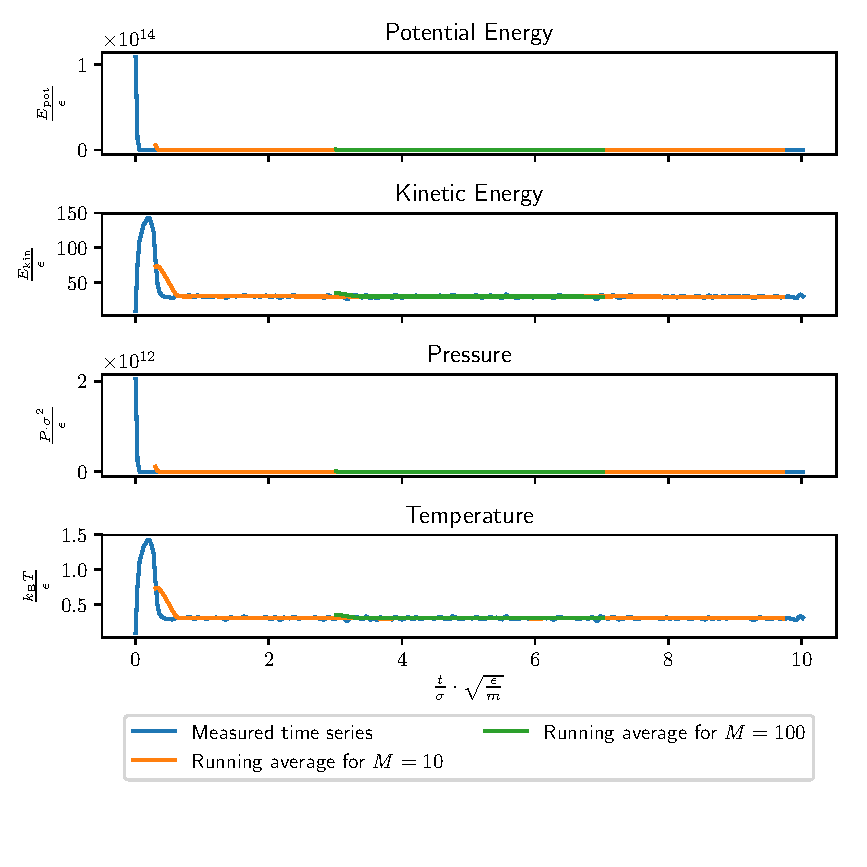
\includegraphics[width=\linewidth]{warm03.pdf}
    \caption{Time evolution of the observables during the warming up for the system with target temperature $T_0 = 0.3\cdot \epsilon\cdot k_\mathrm{B}^{-1}$.}
    \label{fig:figx-1}
\end{figure}
\begin{figure}
        \centering
        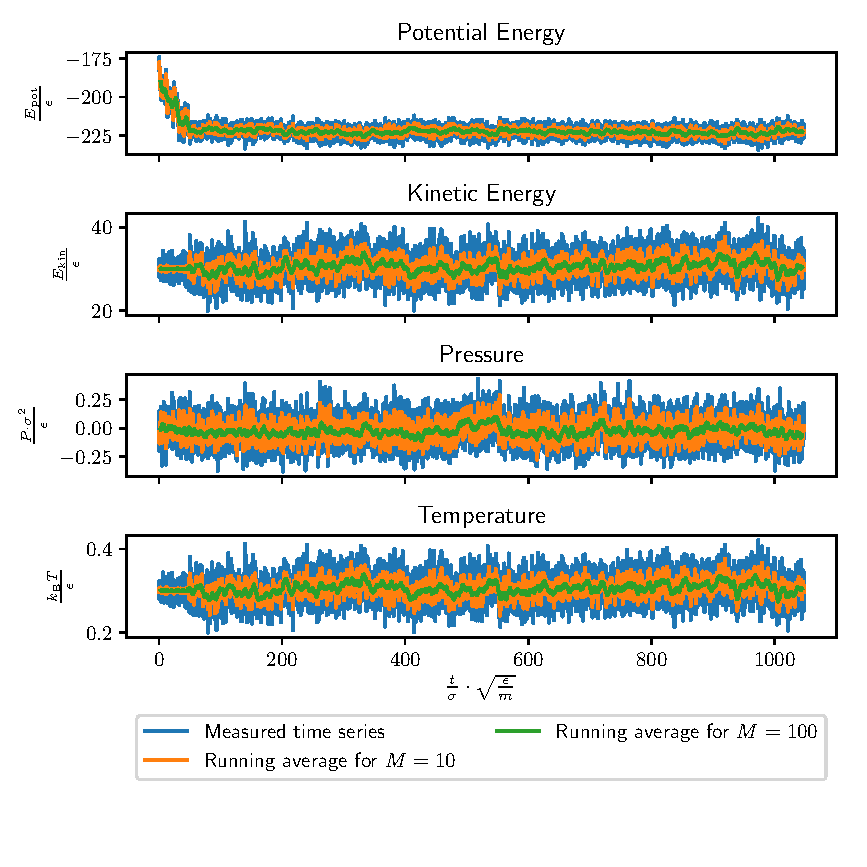
\includegraphics[width=\linewidth]{equi03.pdf}
    \caption{Time evolution of the observables during after warming up for the system with target temperature $T_0 = 0.3\cdot \epsilon\cdot k_\mathrm{B}^{-1}$. During the 5000 time steps in the beginning, the velocity rescaling is turned on.}
    \label{fig:figx0}
\end{figure}
\begin{figure}
        \centering
        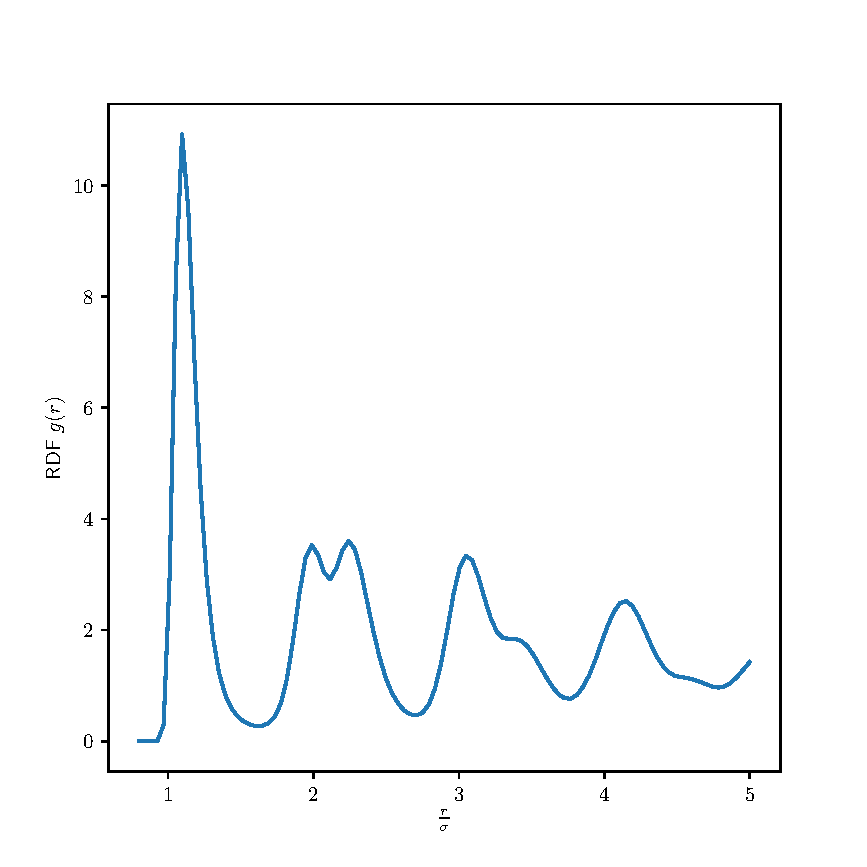
\includegraphics[width=\linewidth]{rdf03.pdf}
    \caption{Equilibrium mean value of the radial distribution function for $k_\mathrm{B}T/\epsilon=0.3$.}
    \label{fig:figx1}
\end{figure}

\newpage
\subsection{$T = 1.0\cdot \epsilon\cdot k_\mathrm{B}^{-1}$}
To warm up the system with random initial positions, a simulation with an initial force capping of $f_\mathrm{max} = 20.0\cdot\epsilon\cdot \sigma^{-1}$ and velocity rescaling was run for 1000 time steps.
A plot of the observables during this warming up is shown in \autoref{fig:figy-1}.
We can see that both pressure and potential energy steeply decrease.
After that, the force capping was removed and the system was simulated for another 6000 time steps with the velocity rescaling still activated. 
In the end, the system was simulated for another 100000 time steps with the velocity rescaling turned off.
A plot of the different observables after the warming up is shown in \autoref{fig:figy0}.
We can see that the system is already equilibrated once the velocity rescaling is turned off. 

The computed equilibrium mean values of the observables are:
\begin{align*}
\left\langle E_\mathrm{pot}/\epsilon \right\rangle &\approx-79.07\\
\left\langle E_\mathrm{kin}/\epsilon\right\rangle &\approx 105.2\\
\left\langle \frac{P\sigma ^2}{\epsilon}\right\rangle &\approx0.3337\\
\left\langle \frac{k_\mathrm{B}T}{\epsilon}\right\rangle &\approx1.052.
\end{align*}
We can see that the mean temperature stays close to the target temperature.

The equilibrium mean value of the radial distribution function for this case is shown in \autoref{fig:figy1}. 
The radial distribution function for this temperature resembles the radial distribution function of a liquid, the oscillations quickly decay for large values of the distance $r$, the function approaches the value 1.
This result indicates that the Lennard-Jones-Fluid forms a liquid phase with short range-order for this temperature.
\begin{figure}
        \centering
        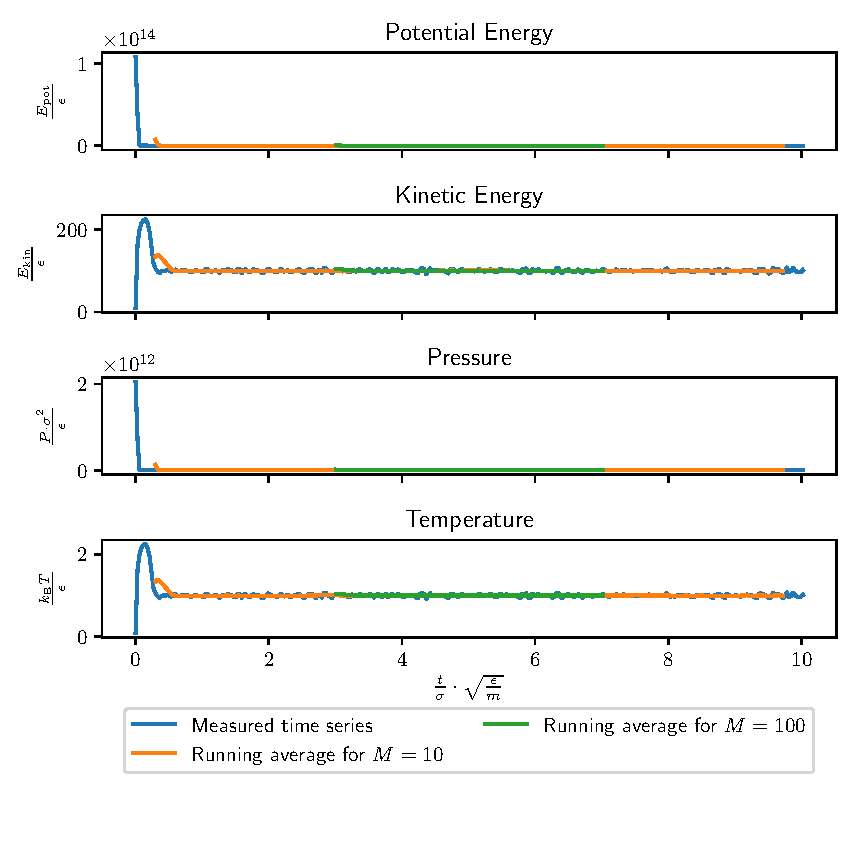
\includegraphics[width=\linewidth]{warm1.pdf}
    \caption{Time evolution of the observables during the warming up for the system with target temperature $T_0 = 1.0\cdot \epsilon\cdot k_\mathrm{B}^{-1}$.}
    \label{fig:figy-1}
\end{figure}
\begin{figure}
        \centering
        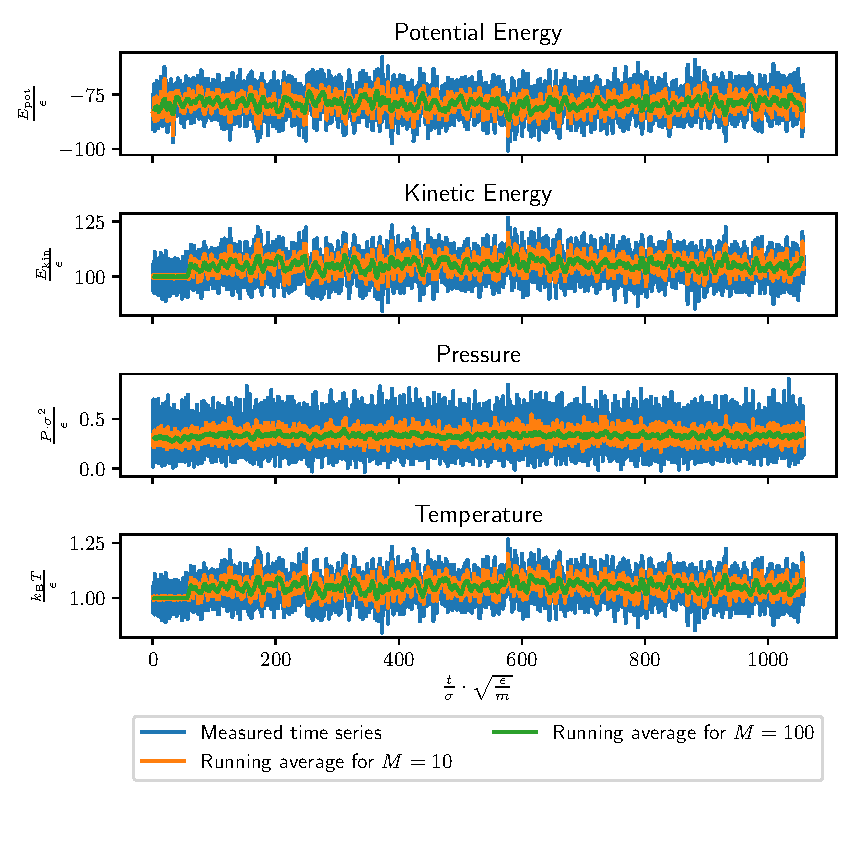
\includegraphics[width=\linewidth]{equi1.pdf}
    \caption{Time evolution of the observables during after warming up for the system with target temperature $T_0 = 1.0\cdot \epsilon\cdot k_\mathrm{B}^{-1}$. During the 6000 time steps in the beginning, the velocity rescaling is turned on.}
    \label{fig:figy0}
\end{figure}
\begin{figure}
        \centering
        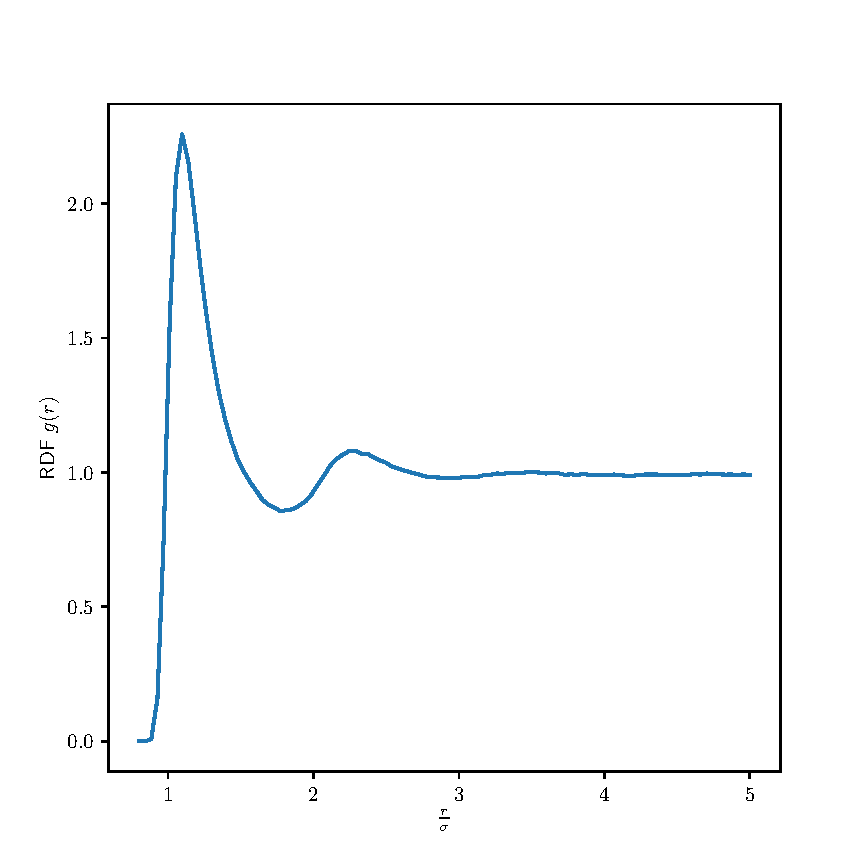
\includegraphics[width=\linewidth]{rdf1.pdf}
    \caption{Equilibrium mean value of the radial distribution function for $k_\mathrm{B}T/\epsilon=1.0$.}
    \label{fig:figy1}
\end{figure}

\newpage
\subsection{$T = 2.0\cdot \epsilon\cdot k_\mathrm{B}^{-1}$}
To warm up the system with random initial positions, a simulation with an initial force capping of $f_\mathrm{max} = 20.0\cdot\epsilon\cdot \sigma^{-1}$ and velocity rescaling was run for 1000 time steps.
A plot of the observables during this warming up is shown in \autoref{fig:figz-1}.
We can see that both pressure and potential energy steeply decrease.
After that, the force capping was removed and the system was simulated for another 6000 time steps with the velocity rescaling still activated. 
In the end, the system was simulated for another 100000 time steps with the velocity rescaling turned off.
A plot of the different observables after the warming up is shown in \autoref{fig:figz0}.
We can see that the system is already equilibrated once the velocity rescaling is turned off. 

The computed equilibrium mean values of the observables are:
\begin{align*}
\left\langle E_\mathrm{pot}/\epsilon \right\rangle &\approx-63.80\\
\left\langle E_\mathrm{kin}/\epsilon\right\rangle &\approx 206.8\\
\left\langle \frac{P\sigma ^2}{\epsilon}\right\rangle &\approx0.8710\\
\left\langle \frac{k_\mathrm{B}T}{\epsilon}\right\rangle &\approx2.068.
\end{align*}
We can see that the mean temperature stays close to the target temperature.

The equilibrium mean value of the radial distribution function for this case is shown in \autoref{fig:figz1}. 
The radial distribution function for this temperature resembles the radial distribution function of a liquid, the oscillations quickly decay for large values of the distance $r$, the function approaches the value 1.
The oscillations decay even faster than in the previous case, this indicates that the fluid approaches the characteristics of a gas as the temperature is increased.
\begin{figure}
        \centering
        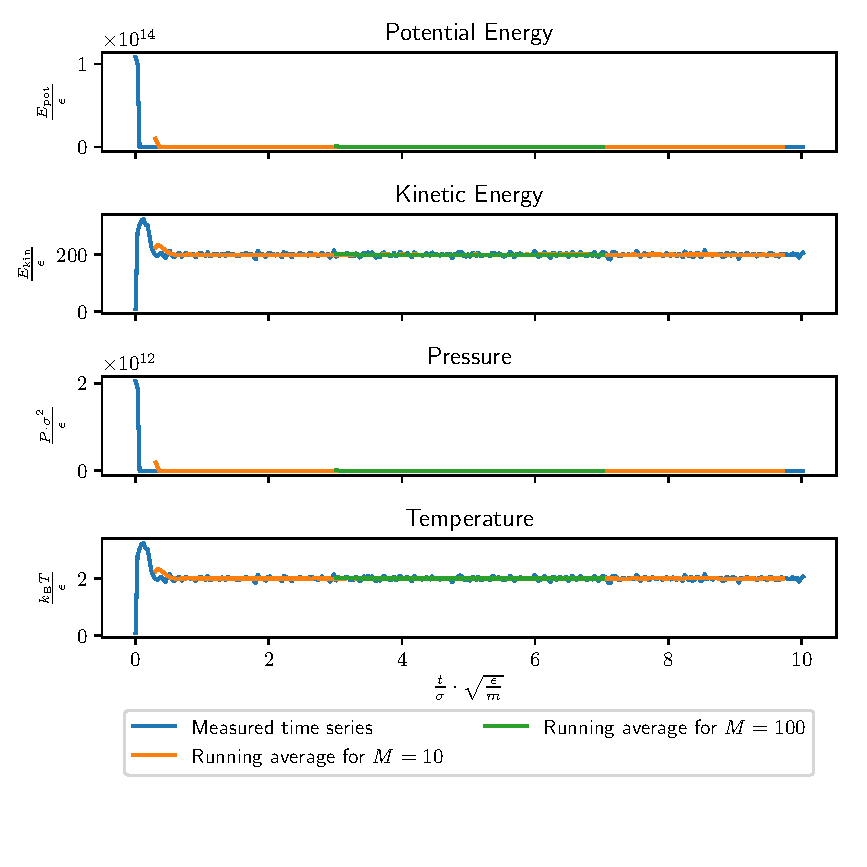
\includegraphics[width=\linewidth]{warm2.pdf}
    \caption{Time evolution of the observables during the warming up for the system with target temperature $T_0 = 2.0\cdot \epsilon\cdot k_\mathrm{B}^{-1}$.}
    \label{fig:figz-1}
\end{figure}
\begin{figure}
        \centering
        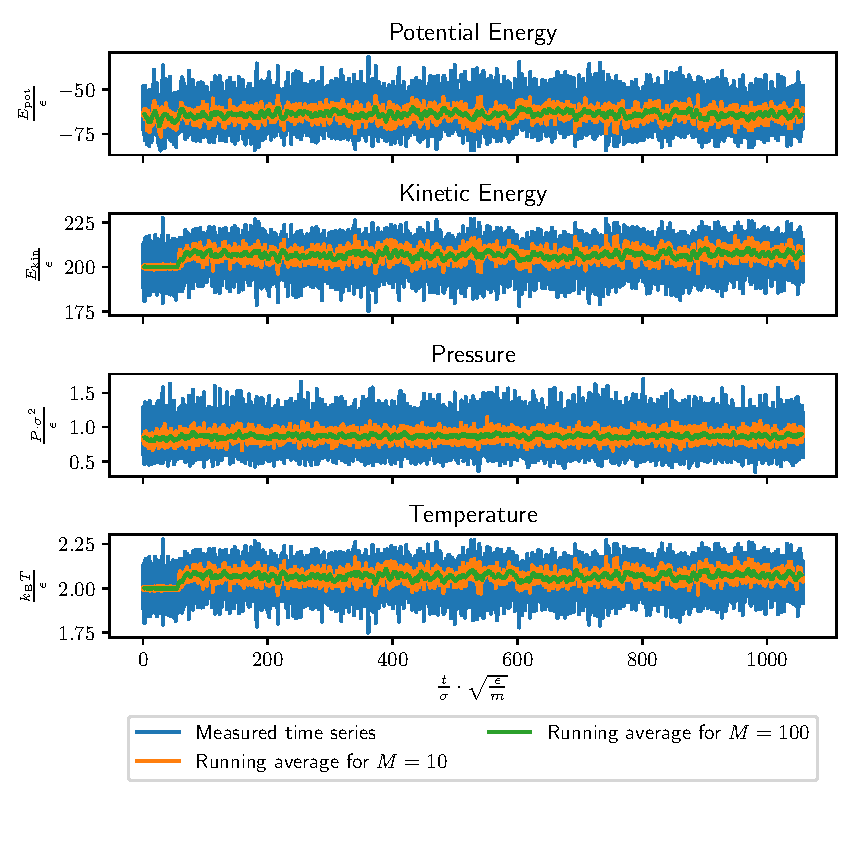
\includegraphics[width=\linewidth]{equi2.pdf}
    \caption{Time evolution of the observables during after warming up for the system with target temperature $T_0 = 2.0\cdot \epsilon\cdot k_\mathrm{B}^{-1}$. During the 6000 time steps in the beginning, the velocity rescaling is turned on.}
    \label{fig:figz0}
\end{figure}
\begin{figure}
        \centering
        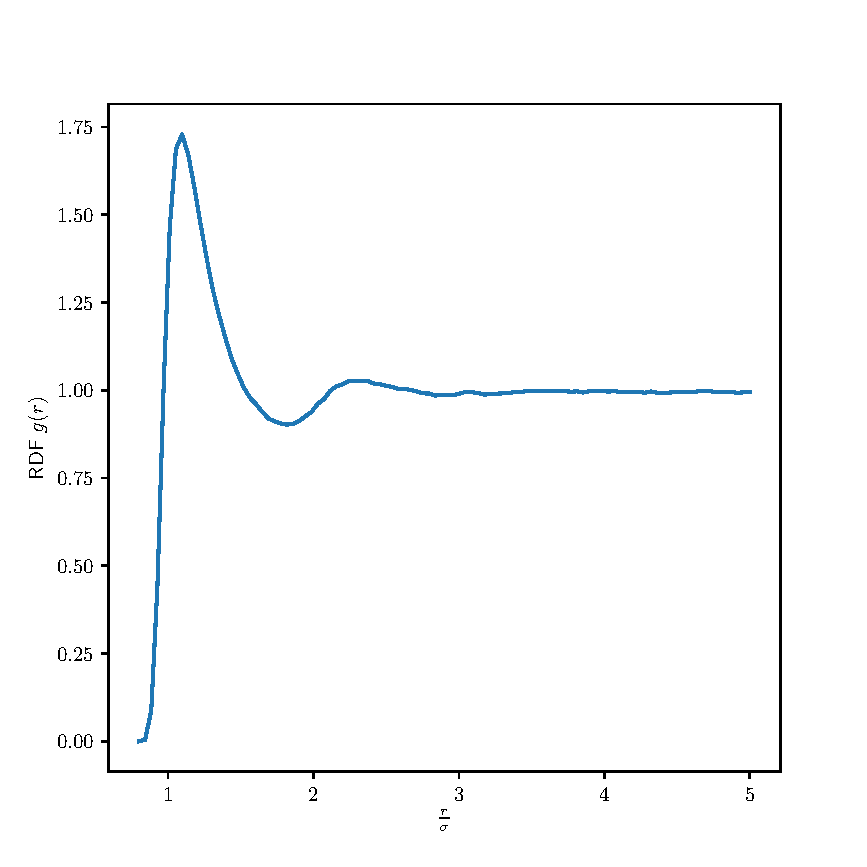
\includegraphics[width=\linewidth]{rdf2.pdf}
    \caption{Equilibrium mean value of the radial distribution function for $k_\mathrm{B}T/\epsilon=2.0$.}
    \label{fig:figz1}
\end{figure}

\newpage
\section{Tail Correction in the Pressure Calculation}
The pressure for a system in $d$ dimensions with volume $V$ can be calculated using the expression
\begin{align}
P = \underbrace{\frac{Nk_\mathrm{B}T}{V}}_{\text{ideal gas contribution}} + \underbrace{\frac{1}{dV}\sum_{i<j}\langle\mathbf{r}_{ij}\cdot\mathbf{F}_{ij}\rangle}_{\text{virial contribution}}.
\end{align}
We can split this expression into a part that corresponds to the system with truncated potentials and a correction $\Delta P$:
\begin{align}
P = \underbrace{\frac{Nk_\mathrm{B}T}{V} + \frac{1}{dV}\sum_{\substack{i<j\\ r_{ij}<r_\mathrm{c}}}\langle\mathbf{r}_{ij}\cdot\mathbf{F}_{ij}\rangle}_{P_\text{truncated}} + \underbrace{\frac{1}{dV}\sum_{\substack{i<j\\ r_{ij}>r_\mathrm{c}}}\langle\mathbf{r}_{ij}\cdot\mathbf{F}_{ij}\rangle}_{\Delta P}.
\end{align}
This leads to the expression
\begin{align}
\Delta P = \frac{1}{3V}\sum_{\substack{i<j\\ r_{ij}>r_\mathrm{c}}}\langle\mathbf{r}_{ij}\cdot\mathbf{F}_{ij}\rangle
\end{align}
for a system in 3 dimensions. The average $\langle\mathbf{r}_{ij}\cdot\mathbf{F}_{ij}\rangle$ can in general be calculated using the appropriate statistical mechanical distribution function (for example the Boltzmann distribution for the canonical ensemble). Using the simplifying assumption that the particle density $\rho\left(\mathbf{r}\right)$ is constant and given by 
\begin{align}
\rho\left(\mathbf{r}\right) = \frac{N}{V}
\end{align}
we can explicitly calculate $\langle\mathbf{r}_{ij}\cdot\mathbf{F}_{ij}\rangle$:
\begin{align}
\begin{split}
\langle\mathbf{r}_{ij}\cdot\mathbf{F}_{ij}\rangle_{r_{ij}>r_\mathrm{c}} &\approx \frac{\rho}{N}\iiint_{V\setminus B_{r_\mathrm{c}}(0)}\mathrm{d}^3r_{ij}\,\mathbf{r}_{ij}\cdot\mathbf{F}_{ij}= \frac{1}{V}\iiint_{V\setminus B_{r_\mathrm{c}}(0)}\mathrm{d}^3r_{ij}\,24\epsilon\left(\frac{2\sigma^{12}}{r_{ij}^{12}}-\frac{\sigma^6}{r_{ij}^6}\right)\\ &
\approx \frac{1}{V}\iiint_{\mathbb{R}^3\setminus B_{r_\mathrm{c}}(0)}\mathrm{d}^3r_{ij}\,24\epsilon\left(\frac{2\sigma^{12}}{r_{ij}^{12}}-\frac{\sigma^6}{r_{ij}^6}\right)= \frac{96\pi\epsilon}{V}\int_{r_\mathrm{c}}^{\infty}\mathrm{d}r_{ij}\,r_{ij}^2\left(\frac{2\sigma^{12}}{r_{ij}^{12}}-\frac{\sigma^6}{r_{ij}^6}\right)\\ &= \frac{96\pi\epsilon\sigma^3}{3V}\left(\frac{2}{3}\left(\frac{\sigma}{r_\mathrm{c}}\right)^9-\left(\frac{\sigma}{r_\mathrm{c}}\right)^3\right)
\end{split}
\end{align}
In the third step we extended the range of integration over $\mathbb{R}^3\setminus B_{r_\mathrm{c}}(0)$, this is approximately equal to the integral over $V\setminus B_{r_\mathrm{c}}(0)$ because the integrand goes to zero like $r_{ij}^{-4}$ as $r_{ij}\rightarrow\infty$. Plugging this expression into the formula for the tail correction results in
\begin{align}
\begin{split}
\Delta P &= \frac{1}{3V}\sum_{\substack{i<j\\ r_{ij}>r_\mathrm{c}}}\langle\mathbf{r}_{ij}\cdot\mathbf{F}_{ij}\rangle = \frac{1}{3V}\cdot\frac{N(N-1)}{2}\cdot \langle\mathbf{r}_{ij}\cdot\mathbf{F}_{ij}\rangle_{r_{ij}>r_\mathrm{c}}\\
&\approx \frac{1}{3V}\cdot\frac{N(N-1)}{2}\cdot\frac{96\pi\epsilon\sigma^3}{3V}\left(\frac{2}{3}\left(\frac{\sigma}{r_\mathrm{c}}\right)^9-\left(\frac{\sigma}{r_\mathrm{c}}\right)^3\right)\\
&\approx \frac{16\pi\rho^2\epsilon\sigma^3}{3}\left(\frac{2}{3}\left(\frac{\sigma}{r_\mathrm{c}}\right)^9-\left(\frac{\sigma}{r_\mathrm{c}}\right)^3\right).
\end{split}
\end{align}
In the third step we made use of the approximation $N(N-1)\approx N^2$ for large $N$.




\end{document}
